\documentclass[12pt]{article}
\usepackage[top=1in, bottom=1in, left=1in, right=1in]{geometry}

\usepackage{setspace}
\onehalfspacing

\usepackage{amssymb}
%% The amsthm package provides extended theorem environments
\usepackage{amsthm}
\usepackage{epsfig}
\usepackage{times}
\renewcommand{\ttdefault}{cmtt}
\usepackage{amsmath}
\usepackage{graphicx} % for graphics files
\usepackage{tabu}

% Draw figures yourself
\usepackage{tikz} 

% writing elements
%\usepackage{mhchem}

\usepackage{paralist}

% The float package HAS to load before hyperref
\usepackage{float} % for psuedocode formatting
\usepackage{xspace}

% from Denovo Methods Manual
\usepackage{mathrsfs}
\usepackage[mathcal]{euscript}
\usepackage{color}
\usepackage{array}

\usepackage[pdftex]{hyperref}
\usepackage[parfill]{parskip}

% math syntax
\newcommand{\nth}{n\ensuremath{^{\text{th}}} }
\newcommand{\ve}[1]{\ensuremath{\mathbf{#1}}}
\newcommand{\Macro}{\ensuremath{\Sigma}}
\newcommand{\rvec}{\ensuremath{\vec{r}}}
\newcommand{\vecr}{\ensuremath{\vec{r}}}
\newcommand{\omvec}{\ensuremath{\hat{\Omega}}}
\newcommand{\vOmega}{\ensuremath{\hat{\Omega}}}
\newcommand{\even}{\ensuremath{\phi^g}}
\newcommand{\odd}{\ensuremath{\vartheta^g}}
\newcommand{\evenp}{\ensuremath{\phi^{g'}}}
\newcommand{\oddp}{\ensuremath{\vartheta^{g'}}}
\newcommand{\Sn}{\ensuremath{S_N} }
\newcommand{\Ye}[2]{\ensuremath{Y^e_{#1}(\vOmega_#2)}}
\newcommand{\sigg}[1]{\ensuremath{\Macro^{g'\rightarrow g}_{s,#1}}}
\newcommand{\psig}{\ensuremath{\psi^g}}
%---------------------------------------------------------------------------
%---------------------------------------------------------------------------
\begin{document}
\begin{center}
{\bf NE 155/255, Fall 2019 \\
Discrete Ordinates, P$_N$, SP$_N$\\
October 07, 2019}
\end{center}

\setlength{\unitlength}{1in}
\begin{picture}(6,.1) 
\put(0,0) {\line(1,0){6.25}}         
\end{picture}

%-----------------------------------------
\subsubsection*{Discrete Ordinates Considerations}

Two main things to consider in discrete ordinates: \textit{quadrature choice} 
and \textit{ray effects}. 

\textbf{Level-symmetric} quadratures use the same set of $N/2$ positive values 
of direction cosines with respect to each of the three axes. That is, for each 
level $n$ we set $\mu_a = \eta_a = \xi_a$. We describe a level $a$ as the 
ordinate set that has cosine $\mu_a$ with respect to the $x$-axis. Note that 
with this setup no axis has preferential treatment. \autoref{fig:levelsym} 
shows $S_6$. We see there are $6/2 = 3$ values of each direction cosine, and 
each one is the same with respect to each axis. We have $N(N+2)$ quadrature
points over the sphere, and that divided by 8 per octant (in this case 48 and
6, respectively). 

\begin{figure}[h!]
    \begin{center}
    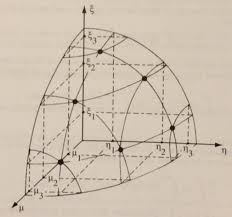
\includegraphics[keepaspectratio, width = 2.5 in]{level-sym}
    \end{center}
    \caption{$S_6$ quadrature}
    \label{fig:levelsym}
\end{figure}

Because of the symmetry constraints, not all of the $\mu_n$ are independent. In 
fact, there is only one degree of freedom because of all of the constraints. 
Choosing $\mu_1$ sets all of the other values as follows:

\[
\mu_i^2 = \mu_1^2 + \frac{2(1 - 3\mu_1^2)}{N-2}(i-1)\:.
\]

See 4-2 of Lewis and Miller for details. Selecting a $\mu_1$ near the poles 
will cause clustering at the poles, and so on. 

Further, we need to select weights to perform the integration. These meet the 
requirement

\[
\sum_{a=1}^{N(N+2)/8} w_a = 1\:.
\]

In the $S_2$ approximation, we only have one choice. For higher values we 
still have some choices. 

A common choice is to choose weights and angles that correctly integrate as 
many Legendre Polynomials as possible. These are shown in in Table 4-1 in L\&M 
and are technically called the $LQ_N$ set. There are other $S_N$ versions that 
have reduced symmetry or relaxation of requirements in other ways. For 
example, if we don't require all of the cosines to lie on the $N/2$ levels we 
can maintain rotational symmetry and have equal weights. 

Another common quadrature is \textbf{Gauss-Legendre}. An $n$-point Gaussian 
quadrature rule is constructed to yield an exact result for polynomials of 
degree $2n - 1$ or less by a suitable choice of the points $x_i$ and weights
$w_i$ for $i = 1, \dots, n$. Common weighting functions include
$w(x)= 1/\sqrt{1-x^2}$ (Chebyshev-Gauss) and $w(x)=e^{-x^{2}}$ (Gauss-Hermite).
In general, the $n$-th polynomial normalized to give $P_n(1) = 1$, the $i$-th 
Gauss node, $x_i$, is the $i$-th root of $P_n$; its weight is given by

\[ 
w_{i}={\frac {2}{\left(1-x_{i}^{2}\right)[P'_{n}(x_{i})]^{2}}}.
\]
    %https://en.wikipedia.org/wiki/Gaussian_quadrature    
    
\textbf{Ray Effects}: ray effects come from the fact that the discrete 
ordinates method is exact at particular angles, but we cannot say anything 
about the accuracy at points off of those angles. Consider a point source in a 
large medium of helium gas. Consider that you've chosen $S_2$. What is the 
flux going to look like? Consider now that you've chosen $S_{14}$. What will the 
flux look like now? It is not very accurate in either case because there is 
nothing to scatter the neutrons from the angles in question. These are ray 
effects; example plots are shown on the following page. 

There are ``fix-up'' solutions to deal with this. The best approach is 
probably generating a first collided flux, stopping the calculation, and 
starting again with the first collision source as the source. This takes the 
point source, smears it across the space, and allows a diffuse starting 
source. This functionally improves quite a bit over straight $S_N$ in 
situations that have unfavorable transport characteristics.

\newpage

\begin{center}
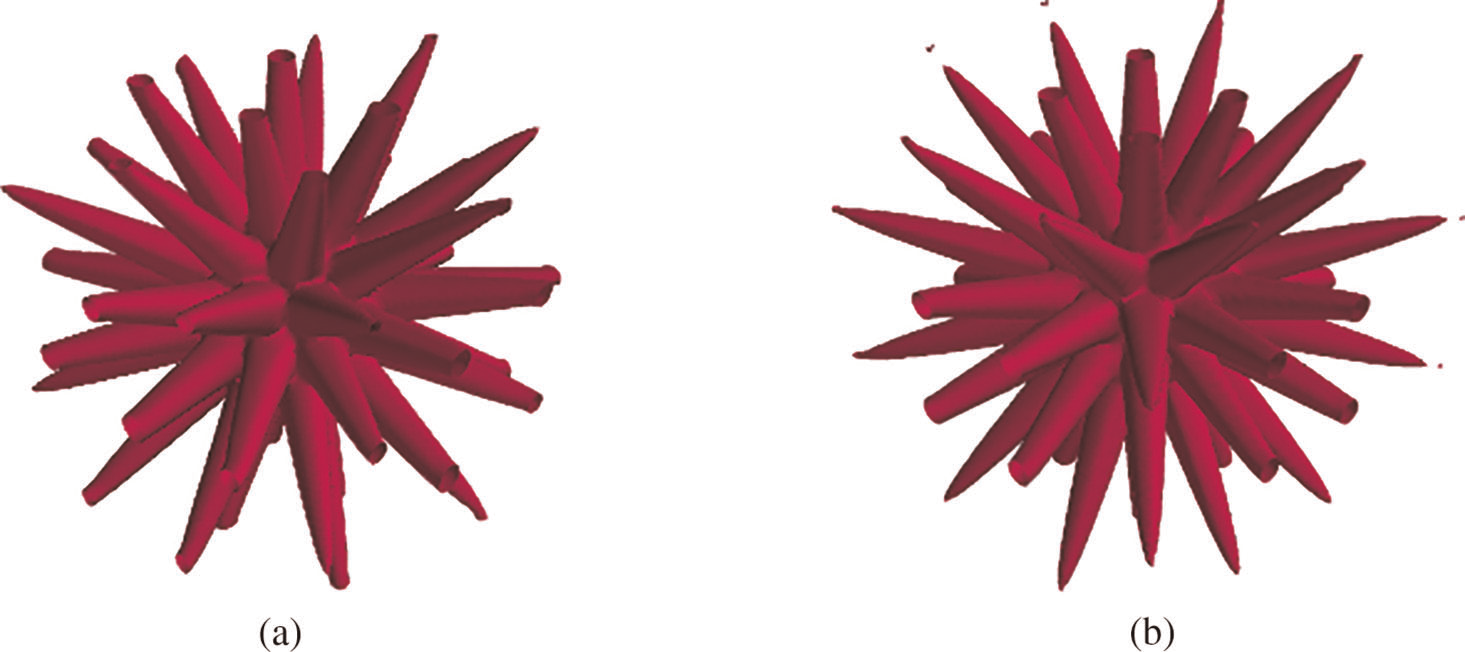
\includegraphics[keepaspectratio, width = \textwidth]{test-001}
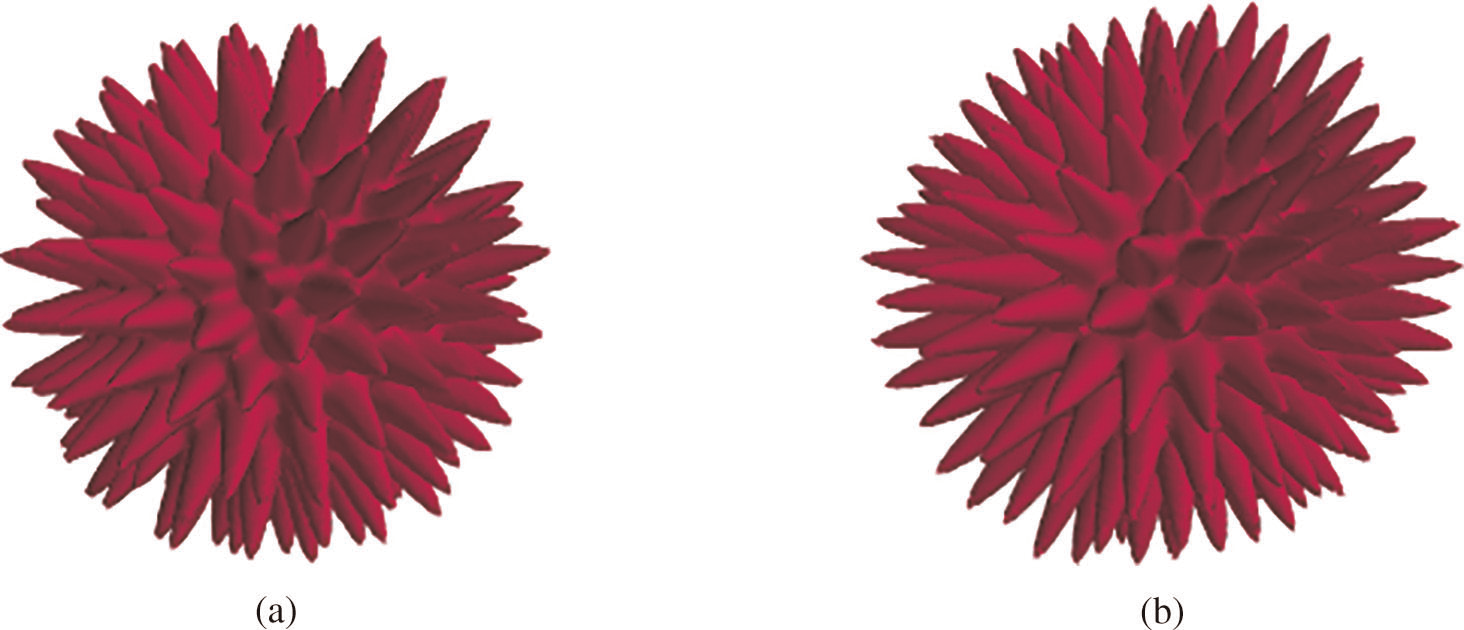
\includegraphics[keepaspectratio, width = \textwidth]{test-002}
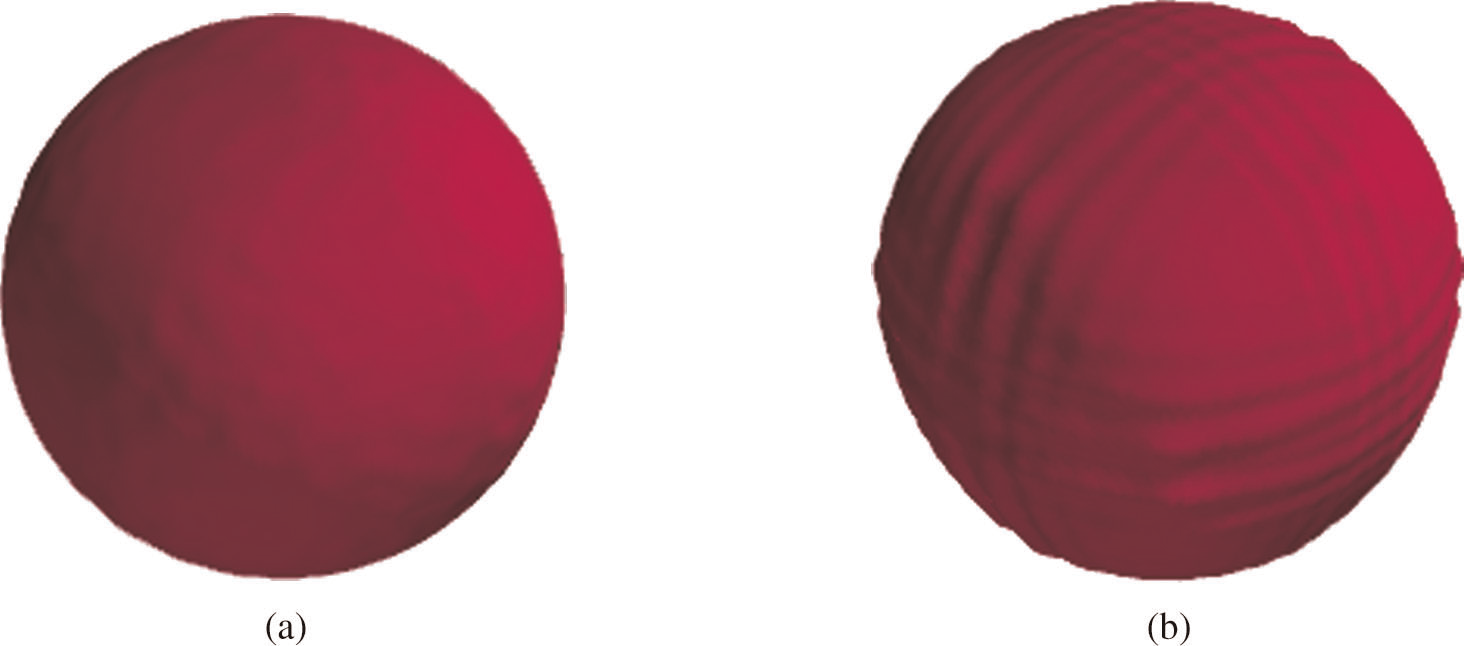
\includegraphics[keepaspectratio, width = \textwidth]{test-003}
\end{center}

\newpage

%-----------------------------------------
%-----------------------------------------
\subsection*{Spherical Harmonics, $P_N$ Method}

As mentioned, the other approach is using Spherical Harmonics more broadly. In 
this method we expand not only scattering and the sources in spherical 
harmonics, but the flux itself. 
% We're going to go through this in 1-D because 
% that's the most approachable way to do this. Frankly, $P_N$ in multi-D is 
% tough and we don't often do it. When we want multi-D we usually go to 
% simplified $P_N$ ($SP_N$). 

We use

\[
\psi(x, \mu) = \sum_{\ell=0}^{\infty} \frac{(2\ell+1)}{4\pi} \phi_\ell(x)P_\ell(\mu)
\]

for the flux solution in total in 1-D. There are some major
\textit{deficiencies} of $P_N$ methods - e.g., we get poor representation of
$\psi$ near vacuum boundaries.

\subsection*{SP$_N$ Equations (general notes)}

The $SP_N$ equations can be understood as a ``super'' diffusion theory.
The structure of the SP$_N$ equations is that of a coupled system of diffusion equations, and the class of problems for which the SP$_N$ equations are accurate encompasses those for which diffusion theory is accurate.

\begin{enumerate}
\item In 1-D planar geometry, SP$_N$ and P$_N$ are identical
\item In multi-D, SP$_N$ form a system of (N + 1) eqs; P$_N$ form a system of (N + 1)$^2$ eqs
\item The SP$_N$ equations have a ``diffusion'' (elliptic) structure; the P$_N$ equations have a more complicated (hyperbolic) mathematical structure.
\item In principle, the 2-D or 3-D SP$_N$ equations can be implemented in a 2-D or 3-D diffusion code without fundamentally rewriting the code.
This is not the case for the P$_N$ equations.
\item The SP$_N$ equations contain more ``transport physics'' than the diffusion equations.
For this reason, solutions of the SP$_N$ equations can contain boundary layers that are not present in P$_1$ solutions.
In order to properly resolve these boundary layers, it may be necessary to use a finer spatial grid for the SP$_N$ equations than for the diffusion equation.
\item In the limit as $N\rightarrow\infty$, the P$_N$ solutions converge to the transport solution.
\item In the limit as $N\rightarrow\infty$, the SP$_N$ solutions don't generally converge to the transport solution unless the underlying problem is 1-D.
Thus, high-order SP$_N$ equations cannot be used to obtain arbitrarily accurate solutions of neutron transport problems in 2- or 3-D.
\item For 3-D problems, the system of P$_N$ equations is much more complicated in structure and greater in number than the system of SP$_N$ equations.
Also, for problems having 1-D symmetry, the P$_N$ and SP$_N$ equations become identical.
For these reasons, it is widely believed that the 3-D SP$_N$ equations can be derived by discarding the proper terms (and equations) from the 3-D P$_N$ equations. However, this has never been shown and the precise relationship between the 3-D P$_N$ and the 3-D SP$_N$ equations is not known.
\end{enumerate}

\subsection*{Approximation Errors}

With discrete ordinates, errors can be removed through spatial integration. 
The physical oscillations in the flux will balance out, and the magnitudes are 
pretty correct. Further, you can visually see ray effects--so you can tell 
that something is going on. You can increase the order, and you can see what 
might or might not be trustworthy. 

With $P_N$ the errors are often in magnitude rather than shape, so it is much 
more difficult to assess whether your solution is correct. (in complex 
geometries it is also sometimes hard to tell for ray effects). 

\end{document}
